\section{SSH model}
Let us start with the simplest topological model Hamiltonian known 
as the Su-Schrieffer-Heeger (SSH) model
which has been used to describe polyacetylene or bi-partite/dimerized (Peierls) lattice
~\cite{su:schrieffer:heeger:prl79}.
%[Barisic et al, 1970, Su et al 1979]. 
The Hamiltonian reads
%
\blgn
\hSSH
&=\sum_{I=1}^{L} [t+(-1)^I\del]c\y_I c\py_{I+1}\non\\
&=\sum_{i=0}^{L-1} (t+\del )c\y_{A\,i} c\py_{B\,i} + \sum_i (t-\del )c\y_{A\,i+1} c\py_{B\,i}+\hc\,\non\\
&\equiv \sum_i [\tp c\y_{A\,i} c\py_{B\,i} + \tm c\y_{A\,i+1} c\py_{B\,i}+\hc]\,.
\label{eq:H:SSH:ispace}
\elgn
Here the lattice consists of two different sublattice sites $A$ and $B$
inside each primitive cell as they associate with two different hopping amplitudes, namely 
$\tm = t-\del$  (representing longer single bond having lesser kinetic energy or hopping for $\del>0$) and $\tp = t + \del$ (representing shorter double bond having higher kinetic energy or hopping for $\del>0$). $\tp$ and $\tm$ are dubbed \emph{intracell} and \emph{intercell} hopping respectively.
%% FIG: SSH chain
% \begin{figure}[!htp]
% \centering
% 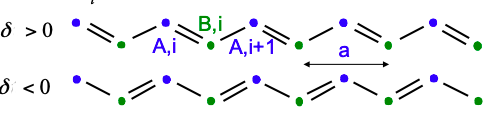
\includegraphics[height=1.5cm,clip]{\FIGDIR/SSH_chains.png}
% \caption{Su-Schrieffer-Heeger (SSH) chains in two different configurations.}
% \end{figure}



Now the Hamiltonian can be written in the matrix
form $\h H= {\bs\Psi}\y {\bf H}  {\bs\Psi}$ with the basis (or spinor)
$\bs{\Psi}\y=[ c\y_{A\,1} c\y_{B\,1} c\y_{A\,2}\cdots ]$. Then the Hamiltonian matrix becomes
\blgn
{\bf H}
=
\bbmat
0      &\tp    &0      &\cdots    &0\\
\tp^*    &0      &\tm  &\cdots   &0\\
\vdots &\vdots &\vdots &\vdots     &0\\
0      &0      &0      &t_{L-1}^*   &0
\ebmat
\elgn
where the $(L-1)$-th hopping amplitude 
$t_{L-1}$ is either $\tp$ or $\tm$ depending on the value of $L$ (even or odd).\\
Note that the above matrix represents the open boundary condition (OBC) where there
exists no left-side hopping from cell 1 (considering cell 2 is on the right of cell 1) and no right-side hopping  from cell $L$. 
However, if the periodic boundary condition (PBC) is applied, i.e. 
left-side hopping from cell 1 is the last cell $L$ and right-side 
hopping from cell $L$ finds the cell 1 back, then the Hamiltonian becomes 
\blgn
{\bf H}
=
\bbmat
0      &\tp    &0      &\cdots &t_L^*\\
\tp^*    &0      &\tm    &\cdots &0\\
\vdots &\vdots &\vdots &\vdots &0\\
t_L      &0      &0      &t_{L-1}  &0
\ebmat
\elgn

To see a demonstration, take a simple example of a 4-site (2-cell) lattice (two $A$-sites + two $B$-sites) with OBC:
\blgn
{\bf H}_{4\times 4}
=
\bbmat
0       &\tp     &0       &0\\
\tp^*   &0       &\tm     &0\\
0       &\tm^*   &0       &\tp\\
0       &0       &\tp^*   &0
\ebmat
\elgn

Then 
\blgn
\h H_{4\times 4}
&= \Psi\y {\bf H}_{4\times 4} \Psi\non\\
&=\bbmat
c\y_{A1} &c\y_{B1} &c\y_{A2} &c\y_{B2}
\ebmat
\bbmat
0       &\tp     &0       &0\\
\tp^*   &0       &\tm     &0\\
0       &\tm^*   &0       &\tp\\
0       &0       &\tp^*   &0
\ebmat
\bbmat
c\py_{A1} \\c\py_{B1} \\c\py_{A2} \\c\py_{B2}
\ebmat\non\\
%
&=\bbmat
c\y_{A1} &c\y_{B1} &c\y_{A2} &c\y_{B2}
\ebmat
\bbmat
\tp c\py_{B1} \\\tp^*c\py_{A1}+\tm c\py_{A2} \\\tm^*c\py_{B1}+\tp c\py_{B2} \\\tp^* c\py_{A2}
\ebmat\non\\
%
&=
\tp c\y_{A1}c\py_{B1} 
+ \tp^* c\y_{B1}c\py_{A1} + \tm c\y_{B1}c\py_{A2}\non\\ 
&\quad + \tm^*c\y_{A2}c\py_{B1} + \tp c\y_{A2}c\py_{B2}
+\tp^* c\y_{B2} c\py_{A2}\,.
\elgn
